\documentclass[12pt]{article}
\usepackage{amsmath, amsfonts, tikz}
\usetikzlibrary{arrows.meta, calc, angles}

\definecolor{lightA}{RGB}{187, 221, 249}
\definecolor{darkA} {RGB}{8,   120, 211}
\definecolor{lightB}{RGB}{204, 140, 242}
\definecolor{darkB} {RGB}{125,   3, 196}

\newcommand{\R}{\mathbb{R}}

\begin{document}
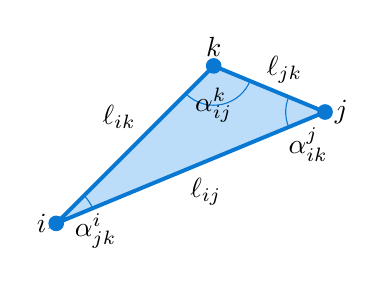
\begin{tikzpicture}
  \coordinate (i) at (-2,0);
  \coordinate (j) at ({sqrt(2)}, {sqrt(2)});
  \coordinate (k) at (0, 2);

  \path[draw, color=darkA, fill=lightA, line width=0.5mm, line cap=round] (i) -- (j) -- (k) -- cycle;

  \node[anchor=east]  at (i) {$i$};
  \node[anchor=west]  at (j) {$j$};
  \node[anchor=south] at (k) {$k$};
  \draw pic[draw=darkA] {angle=j--i--k};
  \draw pic[draw=darkA] {angle=k--j--i};
  \draw pic[draw=darkA] {angle=i--k--j};

  \node at (-1.5, -0.1) {$\alpha_{jk}^i$};
  \node at (0, 1.5) {$\alpha_{ij}^k$};
  \node at (1.2, 1.0) {$\alpha_{ik}^j$};

  \node at (-1.2, 1.35) {$\ell_{ik}$};
  \node at (0.9, 1.95) {$\ell_{jk}$};
  \node at (-0.1, 0.4) {$\ell_{ij}$};

  \node[circle, fill=darkA, inner sep=2pt] at (i) {};
  \node[circle, fill=darkA, inner sep=2pt] at (j) {};
  \node[circle, fill=darkA, inner sep=2pt] at (k) {};

\end{tikzpicture}

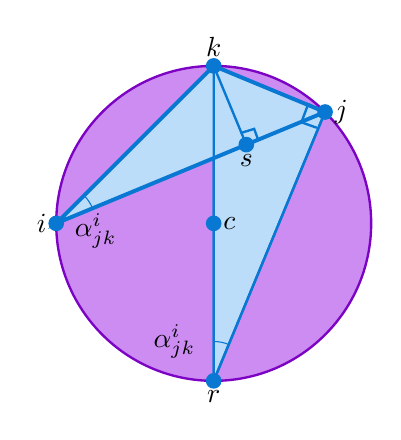
\begin{tikzpicture}
  \coordinate (i) at (-2,0);
  \coordinate (j) at ({sqrt(2)}, {sqrt(2)});
  \coordinate (k) at (0, 2);
  \coordinate (c) at (0, 0);
  \coordinate (r) at (0, -2);
  \def\x{{ 4 * sqrt(2) / (2 + (2 + sqrt(2)) * (2 + sqrt(2))) }};
  \def\y{{(4 * sqrt(2) / (2 + (2 + sqrt(2)) * (2 + sqrt(2))) + 2) * sqrt(2) / (sqrt(2) + 2) }};
  \def\xx{{ 4 * sqrt(2) / (2 + (2 + sqrt(2)) * (2 + sqrt(2)))  + 0.15}};
  \def\yy{{(4 * sqrt(2) / (2 + (2 + sqrt(2)) * (2 + sqrt(2))) + 2) * sqrt(2) / (sqrt(2) + 2) + sqrt(2) / (sqrt(2) + 2) * 0.15}};
  \def\xxx{{ 4 * sqrt(2) / (2 + (2 + sqrt(2)) * (2 + sqrt(2)))  + 0.1}};
  \def\yyy{{(4 * sqrt(2) / (2 + (2 + sqrt(2)) * (2 + sqrt(2))) + 2) * sqrt(2) / (sqrt(2) + 2) + 0.2}};
  \def\xxxx{{ 4 * sqrt(2) / (2 + (2 + sqrt(2)) * (2 + sqrt(2))) - 0.15 * (sqrt (2)) / (sqrt(2) + 2)}};
  \def\yyyy{{(4 * sqrt(2) / (2 + (2 + sqrt(2)) * (2 + sqrt(2))) + 2) * sqrt(2) / (sqrt(2) + 2) + 0.15}};
  \coordinate (s) at (\x, \y);
  \coordinate (ss) at (\xx, \yy);
  \coordinate (sss) at (\xxx, \yyy);
  \coordinate (ssss) at (\xxxx, \yyyy);

  \draw[fill=lightB, draw=darkB, line width=0.3mm] (0,0) circle (2);
  \path[draw, color=darkA, fill=lightA, line width=0.3mm, line cap=round] (j) -- (r) -- (k) -- cycle;
  \path[draw, color=darkA, fill=lightA, line width=0.5mm, line cap=round] (i) -- (j) -- (k) -- cycle;
  \draw[color=darkA, line width=0.3mm, line cap=round] (j) -- (r) -- (k) -- cycle;
  \draw[color=darkA, line width=0.3mm, line cap=round] (s) -- (k);
  \draw[color=darkA, line width=0.3mm, line cap=round] (ssss) -- (sss) -- (ss);
  \draw[color=darkA, line width=0.3mm] (1.414, 1.414) -- (1.2, 1.514) -- (1.114, 1.284) -- (1.31, 1.214);

  \node[anchor=east]  at (i) {$i$};
  \node[anchor=west]  at (j) {$j$};
  \node[anchor=south] at (k) {$k$};
  \node[anchor=west]  at (c) {$c$};
  \node[anchor=north] at (r) {$r$};
  \node[anchor=north] at (s) {$s$};
  \node at (-1.5, -0.1) {$\alpha_{jk}^i$};
  \node at (-0.5, -1.5) {$\alpha_{jk}^i$};

  \node[circle, fill=darkA, inner sep=2pt] at (i) {};
  \node[circle, fill=darkA, inner sep=2pt] at (j) {};
  \node[circle, fill=darkA, inner sep=2pt] at (k) {};
  \node[circle, fill=darkA, inner sep=2pt] at (c) {};
  \node[circle, fill=darkA, inner sep=2pt] at (r) {};
  \node[circle, fill=darkA, inner sep=2pt] at (s) {};

  \draw pic[draw=darkA] {angle=j--i--k};
  \draw pic[draw=darkA] {angle=j--r--k};
\end{tikzpicture}

\end{document}
